\chapter{Research development and prototype}\label{chap:3}

\section{From the original brief to a shared task family}\label{sec:3-1}

The project began with a familiar physical construction task as a basis for investigating collaboration in VR. Early planning used Tangram to examine communication, coordination and awareness before moving into a virtual environment. The first physical test plan recorded prospective sample ranges, timing and ordering arrangements. The final study procedure is described in Chapter~\ref{chap:4}. [\hyperlink{src:D28}{D28}, \hyperlink{src:D29}{D29}, \hyperlink{src:D30}{D30}]

During the first semester, supervisor discussions encouraged an explicit research aim alongside the technical prototype. The June discussion considered how participants might work on separate parts or jointly take responsibility for a task. This kept the project open to different forms of cooperation rather than requiring both people to touch the same object. It also established why observing the organisation of work would be relevant to a viewpoint study. [\hyperlink{src:D34}{D34}, \hyperlink{src:D35}{D35}]

The early expectations concerned both spatial understanding and the organisation of work. In an email of 19 August, the researcher proposed that a shared external view might make the overall workspace and the partner's activity easier to understand, while making individual working areas and agency less clearly separated. First-person viewing was expected to allow clearer personal areas or divisions of work. These possibilities guided what to observe as the project developed. The study retained the exploratory aim discussed with the supervisor: to understand differences in collaborative activity through a working prototype. [\hyperlink{src:D32}{D32}, \hyperlink{src:D34}{D34}, \hyperlink{src:D31}{D31}]

The August plan developed the idea of shared spatial representations. It considered physical Tangram, VR Tangram for familiarisation and a more open VR construction task, such as building a vehicle. The accompanying email recognised that spatial overlap or activity alone would be insufficient as a measure of collaboration quality. The present analysis follows that concern by examining the sequence and meaning of actions rather than their volume. [\hyperlink{src:D31}{D31}, \hyperlink{src:D32}{D32}]

The supervisor's response on 20 August explained why using a common task family would strengthen comparison. Changing from physical Tangram to an entirely different VR activity would introduce task differences alongside the intended viewpoint comparison. The 1 September meeting revisited the alternatives of using construction blocks in every condition or Tangram in every condition. Tangram was selected to focus the implementation on the original collaboration question. [\hyperlink{src:D33}{D33}, \hyperlink{src:D36}{D36}]

\begin{figureunit}{3-1}
The same feedback questioned the assumption that a collaborative task must be indivisible. Participants can work on separate parts and still choose when to work together. An intermediate test table contained eight combinations, including prescribed roles and free collaboration. After trying the procedure, the researcher removed prescribed roles because they made the testing more complicated and restricted how partners organised the task. The final design let both participants manipulate pieces and negotiate their own next actions. This made temporary division, assistance and changes of initiative available for observation. [\hyperlink{src:D37}{D37}, \hyperlink{src:D69}{D69}, \hyperlink{src:D38}{D38}]

\par\begingroup
\centering
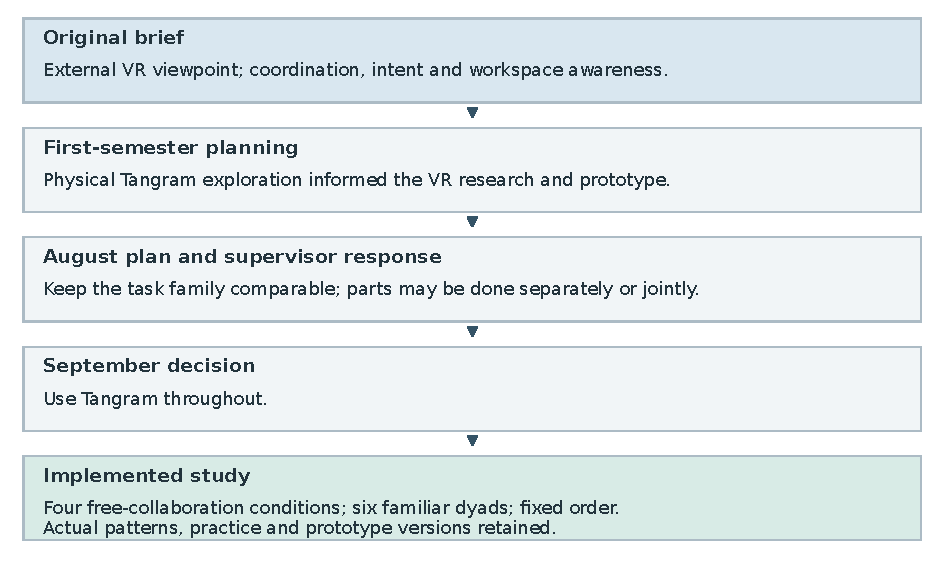
\includegraphics[width=\linewidth,height=95mm,keepaspectratio]{assets/figures/Figure3_1_research_development.pdf}
\captionof{figure}[Development of the research focus and study design.]{Development of the research focus and study design. The August feedback called for a comparable task family while retaining the possibility of individual and joint work. The September discussion selected Tangram across the tasks. The final four-condition study is shown separately from those earlier plans. Sources: original project brief, early study plan, August thesis plan and supervisor response, 1 September meeting transcript, and final study procedure.}\label{fig:3-1}
\par\endgroup
\end{figureunit}




\section{The physical and virtual arrangements}\label{sec:3-2}

\begin{figureunit}{3-2}
The four conditions changed the visual access to a shared Tangram workspace while retaining a common construction task. Figure~\ref{fig:3-2} shows the physical apparatus and the virtual display arrangements. In each condition both partners could manipulate pieces and propose placements. The arrangements are described separately because a shared image and an intuitive mapping from hand movement to that image are different properties. [\hyperlink{src:D24}{D24}, \hyperlink{src:D38}{D38}, \hyperlink{src:D41}{D41}]

\par\begingroup
\centering
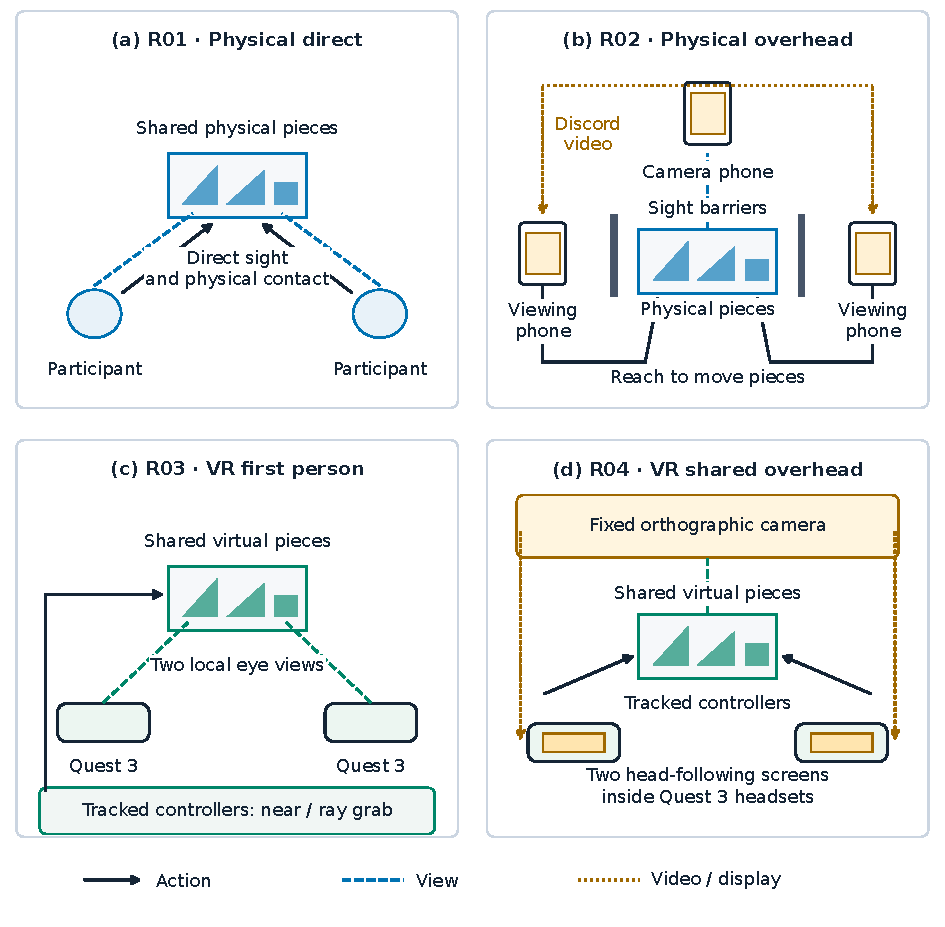
\includegraphics[width=\linewidth,height=140mm,keepaspectratio]{assets/figures/Figure3_2_apparatus.pdf}
\captionof{figure}[Apparatus and view mapping in the four study conditions (schematic, not to scale).]{Apparatus and view mapping in the four study conditions (schematic, not to scale). R02 uses one overhead camera phone and two participant viewing phones, with barriers blocking direct sight of the physical pieces. R03 provides local first-person views in two networked Quest 3 headsets. R04 displays the fixed overhead camera on a head-following screen inside each headset while retaining tracked controller manipulation. The VR schematic represents the shared-target collection arrangement used for G02--G06; the earlier G01 target arrangement is described in Section~\ref{sec:3-3}.}\label{fig:3-2}
\par\endgroup
\end{figureunit}

\begin{samepage}
In R01, physical direct viewing, participants looked directly at and moved seven physical pieces in the shared workspace. In R02, physical overhead video, one smartphone mounted above the table filmed the pieces. A Discord video call sent this live overhead feed to two other smartphones, one for each participant. Barriers blocked direct sight of the workspace. Participants watched their own phone while reaching into the shared physical workspace to move the real pieces. The setup changed visual access while retaining physical contact with the pieces. [\hyperlink{src:D24}{D24}, \hyperlink{src:D39}{D39}]
\par\end{samepage}

The two VR conditions used two networked Meta Quest 3 headsets running the Unity multiplayer Tangram prototype. Both participants manipulated the same seven virtual pieces using tracked controllers, with near and ray grabbing available. The host maintained the shared session and recorded the event stream. Software host and guest endpoints were mapped to the same participant numbers used in the recordings and questionnaires. [\hyperlink{src:D24}{D24}, \hyperlink{src:D39}{D39}, \hyperlink{src:D25}{D25}]

In R03, first-person VR, the participant viewed the scene from their own tracked perspective. In R04, shared overhead VR, a fixed orthographic camera provided a top view of the workspace on a virtual screen that followed the head and replaced the ordinary first-person scene. The screen was inside the headset. Controller tracking continued in the shared three-dimensional space, so the control mechanism remained spatial even though the displayed workspace was a top projection. [\hyperlink{src:D39}{D39}, \hyperlink{src:D40}{D40}, \hyperlink{src:D41}{D41}]

For the shared-target implementation used in the recorded G02--G06 sessions, both endpoints received the same world-oriented overhead image. Moving the head moved the display surface, but moving around the table did not rotate the overhead camera to match the participant. The target orientation, camera orientation and direction of the participant's own movements were therefore recorded as separate aspects of the setup. Participants sometimes changed position to find a more comfortable relation between what they saw and how they moved. This was a self-initiated adaptation described in the process records. [\hyperlink{src:D25}{D25}, \hyperlink{src:D41}{D41}, \hyperlink{src:D46}{D46}]

\par\addvspace{8pt}
\noindent\begin{minipage}{\linewidth}
\begingroup
\centering
\setstretch{1}
\fontsize{10}{12.3}\selectfont
\setlength{\tabcolsep}{2.2pt}
\renewcommand{\arraystretch}{1.18}
\captionof{table}[Implemented research conditions in fixed order.]{Implemented research conditions in fixed order.}\label{tab:3-1}
\begin{tabular}{@{}>{\raggedright\arraybackslash}p{13.729mm}>{\raggedright\arraybackslash}p{42.169mm}>{\raggedright\arraybackslash}p{101.009mm}@{}}
\toprule
\textbf{Round} & \textbf{Viewing} & \textbf{Manipulation and scope} \\
\midrule
R01 & Physical direct & Direct sight of a shared physical workspace; both partners move real pieces. \\
\addlinespace[3pt]
R02 & Physical overhead video & One overhead smartphone streams through Discord to two participant phones; barriers block direct sight; both move real pieces. \\
\addlinespace[3pt]
R03 & VR first person & Two Quest 3 headsets; local tracked views of shared virtual pieces; near and ray grabbing. \\
\addlinespace[3pt]
R04 & VR shared overhead & A world-fixed orthographic image appears on a head-following screen in each headset; controllers remain tracked in the shared 3D workspace. \\
\bottomrule
\end{tabular}
\par\endgroup
\end{minipage}\par\addvspace{8pt}




\section{Prototype changes and exposure history}\label{sec:3-3}

Target presentation changed during development. The first G01 recording used targets oriented to individual users. G02--G06 used the revised shared-target arrangement. The recorded configuration includes a fixed shared target, zero guest-specific optical rotation and manual ending without a time limit. After this iteration, G01 also experienced the full revised procedure. The pair preferred the new version but chose not to record the procedure again; their feedback is retained as a development observation. [\hyperlink{src:D43}{D43}, \hyperlink{src:D25}{D25}, \hyperlink{src:D74}{D74}]

Target patterns, VR experience and familiarisation varied between pairs. G01's candle-orientation discussion occurred during practice and informed development. G02's VR recordings were collected later using new target patterns that the pair had not previously solved. They are included with the other five pairs in the process analysis. Familiarisation was also part of the procedure for the other groups. [\hyperlink{src:D50}{D50}, \hyperlink{src:D17}{D17}, \hyperlink{src:D74}{D74}]

The original plan anticipated viewpoint switching. In the implemented formal rounds, the viewpoint remained locked to the designated condition. During G06's first-person candle task, a participant requested another view and the pair continued in first-person VR. View changes in preparation or between attempts form part of the exposure history. [\hyperlink{src:D14}{D14}, \hyperlink{src:D15}{D15}]


